\documentclass[10pt,oneside]{amsart}
\renewcommand{\familydefault}{\sfdefault}
\usepackage{mathpazo}
\usepackage[letterpaper]{geometry}
\geometry{verbose,tmargin=0.5in,bmargin=0.5in,lmargin=1in,rmargin=1in}
\setlength{\parskip}{\medskipamount}
\setlength{\parindent}{0pt}
\usepackage{booktabs}
\usepackage{amsthm}
\usepackage{graphicx}
\usepackage{setspace}
\usepackage{amssymb}
\usepackage{gensymb}
\usepackage{textcomp}
\usepackage{xcolor}
\usepackage{bm}

%\pagestyle{plain}
\raggedright

\begin{document}

\thispagestyle{empty}









\newpage
\textbf{Pumped Storage Example  (Series Pipeline)}

\begin{center}
	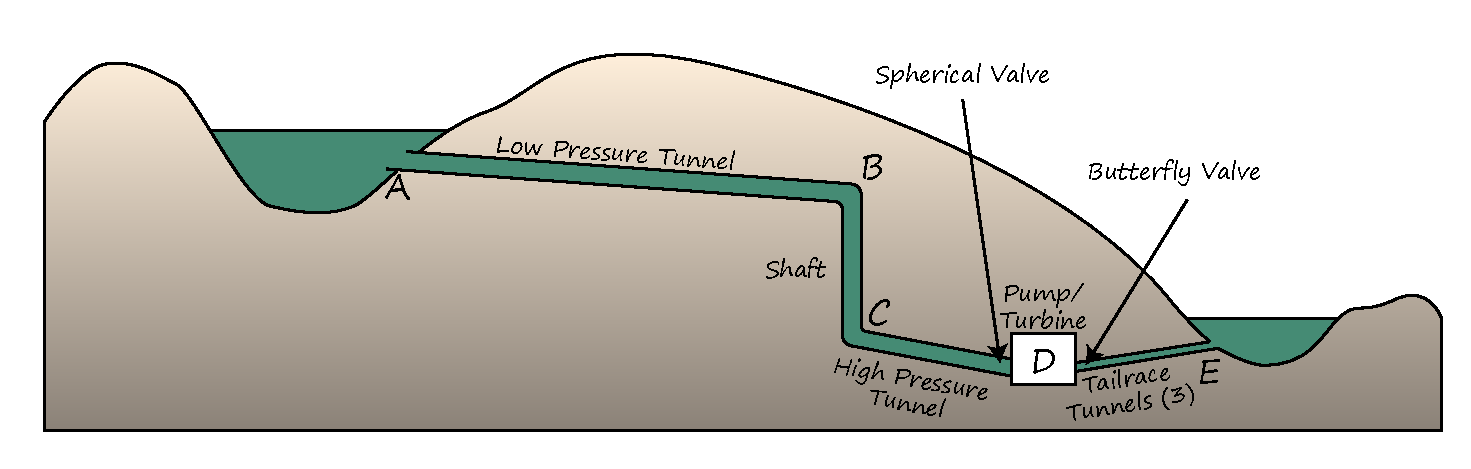
\includegraphics[scale=0.7]{../../figs/07SeriesPipeline/pumpedStorage}
\end{center}

The system illustrated is a pumped storage system. During periods of high demand for electricity, water flows from the
upper lake and drives the turbine at $D$. (During periods of low demand when electricity is cheap, such as at
night-time, $D$ acts as a pump and pumps water back up to the upper lake.)
\par\medskip
At times of maximum demand, the system has a maximum volume flow rate of $420\;\mathsf{m^3/s}$. Base your
calculations on this flow. The water is at $10\text{\textcelsius}$, with a specific gravity of $1.0$ and a viscosity
of $0.0013\;\mathsf{Pa\cdot s}$.
\par\medskip
The difference in elevation between the surfaces of the two lakes is $542\text{
	m}$. \par\medskip
The low pressure tunnel from $A$ to $B$ is $1700\text{ m}$ in length, has a diameter of $10.5\text{ m}$
and is lined with concrete. ($\epsilon=1.2\times10^{-3}\text{ m}$.)
\par\medskip
The shaft and high pressure tunnel from $B$ to $D$ is $1140\text{ m}$ in length, has a diameter of $10.5\text{ m}$ and
is lined with welded steel ($\epsilon=4.6\times10^{-5}\text{ m}$.)
\par\medskip
(Notice that tunnel $AB$ and tunnel $BD$ are of different materials so their losses must be calculated separately!)
\par\medskip
There are {\Large\textbf{three}} tailrace tunnels from the turbine to the lower reservoir with the flow equally
distributed between them (that is, each tailrace tunnel has a flow of $140\;\mathsf{m^3/s}$). Each tailrace tunnel is $382\text{ m}$ in
length, has a diameter of $8.5\text{ m}$ and is lined with concrete. ($\epsilon=1.2\times10^{-3}\text{ m}$.)

(Calculate the headlosses for one tailrace tunnel and simply multiply that loss by three to get the total
tailrace tunnel losses.)

\par\medskip
The entrance to the low pressure tunnel at the upper lake has an equivalent length ratio of $Le/D=420$. The bends at
$B$ and $C$ are in the steel pipe and each have at equivalent length ratio of $16$. A spherical valve at the
inlet of the turbine that shuts off flow when the turbines are not operating is hydraulically efficient and has no
losses associated with it. Each tailrace tunnel contains a butterfly valve ($Le/D=20$).
\par\medskip
At maximum capacity, the turbine outputs $1800 \text{ MW}$. Determine the efficiency of the turbine at this output.




\vfill
\newpage



\textbf{Solution}: (Text in \textcolor{red}{red} is	explanatory and is not required in your solution.)

\textcolor{red}{Series pipelines problems require finding the head losses, both due to friction and minor
	losses, to find the total head loss in the system. Then the General Energy Equation is applied, using the combined head losses already
calculated.}

\textbf{Pipe AB}

\textcolor{blue}{\em Velocity and velocity head in the $10.5$ m diameter tunnel}:\\

\[
	v = \frac{Q}{A} = \frac{420\mathsf{\;m^3/s}}{\pi(10.5\mathsf{ m})^2/4}=4.8504\mathsf{\ m/s}
\]

\[
	\frac{v^2}{2g} = \frac{(4.8504\mathsf{\;m/s})^2}{2\times9.81\mathsf{\;m/s^2}} = 1.1991\mathsf{\; m}
\]

\textcolor{blue}{\em Reynolds Number, relative roughness and friction factors for tunnel AB}:

\[
	N_R = \frac{vD\rho}{\eta} =
	\frac{4.8504\mathsf{\;m/s\;}\times10.5\mathsf{\;m\;}\times1000\mathsf{\;kg/m^3}}{0.0013\;\mathsf{Pa\cdot s}} =
	39176000
\]

\[
	\frac{D}{\epsilon_{concrete}} = \frac{10.5\;\text{m}}{1.2\times10^{-3}\text{ m}} = 8750
\]

\textcolor{blue}{\em Using Swamee-Jain}:
\[
	f = \frac{0.25}{\left[\log\left(\frac{1}{3.7(D/\epsilon)}+\frac{5.74}{N_R^{0.9}}\right)\right]^2} =
	\frac{0.25}{\left[\log\left(\frac{1}{3.7(8750)}+\frac{5.74}{3917600^{0.9}}\right)\right]^2}=0.012354
\]

\[
	f_T = \frac{0.25}{\left[\log\left(\frac{1}{3.7(8750)}\right)\right]^2} = 0.012290
\]

\textcolor{red}{$f_T$ can be found in a number of ways: from the Moody Diagram using a Reynolds Number of $10^8$ (that
	is, the right hand edge of the diagram), from the Swamee-Jain using a Reynolds Number of $10^8$, or from the
	Swamee-Jain omitting the $5.74/N_R^{0.9}$ term altogether since this term is very small. The Swamee-Jain value for $f_T$ in this problem is $0.012318$ with $N_R=10^8$
	or $0.012290$ omitting the $5.74/N_R^{0.9}$ term. Given that the Swamee-Jain formula is an approximation of the Moody
	Diagram and that we can't distinguish between $0.012318$ and $0.012290$ on the Moody Diagram, the difference may be
ignored.}

\textcolor{blue}{\em Using Moody}:
Readings from the Moody Diagram for $f$ and $f_T$ are both approximately $0.0123$. This is the
value I shall use.

\textcolor{blue}{\em Losses for tunnel AB}:
\begin{align*}
	\text{Entrance Losses:}\qquad h_{L} & = k\frac{v^2}{2g} =                        
	f_T\left(\frac{Le}{D}\right)\frac{v^2}{2g}=0.0123\times 420\times 1.1991 = 6.1946\\
	\text{Friction Losses:}\qquad h_{L} & =  f\cdot\frac{L}{D} \cdot\frac{v^2}{2g} = 
	0.0123\cdot\frac{1700}{10.5}\cdot1.1991 = 2.3879\\\\
	h_{L_{AB}}                          & = 6.1946+2.3879 = 8.5825\;\text{m}         
\end{align*}

\textbf{Tunnel BCD}

\textcolor{blue}{\em Velocity, velocity head and Reynolds Number for tunnel BCD } \textcolor{red}{ (unchanged from
tunnel AB calculations above since the dimensions are unchanged)}:

\[
	v = 4.8504\mathsf{\ m/s},\;\frac{v^2}{2g} = 1.1991\mathsf{\; m},\; N_R = 39176000
\]

\textcolor{blue}{\em Relative roughness and friction factors for tunnel BCD}:

\[
	\frac{D}{\epsilon_{steel}} = \frac{10.5\;\text{m}}{4.6\times10^{-5}\text{ m}} = 228260
\]

\textcolor{blue}{\em Using Swamee-Jain}:
\[
	f = \frac{0.25}{\left[\log\left(\frac{1}{3.7(D/\epsilon)}+\frac{5.74}{N_R^{0.9}}\right)\right]^2} =
	\frac{0.25}{\left[\log\left(\frac{1}{3.7(228260)}+\frac{5.74}{39176000^{0.9}}\right)\right]^2}=0.0077125\approx 0.0077
\]

\[
	f_T = \frac{0.25}{\left[\log\left(\frac{1}{3.7(228260)}\right)\right]^2} = 0.0071174\approx 0.0071
\]



\textcolor{blue}{\em Using Moody}:
Readings for $f$ and $f_T$ lie outside the boundary of the Moody Diagram (because of the relatively smooth tunnel and
high Reynolds Number) but extrapolating would seem to indicate (roughly) that $f\approx 0.0075$ and $f_T\approx
0.0070$. In this case, the Swamee-Jain is probably more accurate than my imperfect extrapolation.

\textcolor{blue}{\em Losses for tunnel BCD}:
\begin{align*}
	\text{2 bends:}\qquad h_{L}         & = 2k\frac{v^2}{2g} =                      
	2f_T\left(\frac{Le}{D}\right)\frac{v^2}{2g}=2\times 0.0071\times 16\times 1.1991 = 0.27244\\
	\text{Friction Losses:}\qquad h_{L} & = f\cdot\frac{L}{D} \cdot\frac{v^2}{2g} = 
	0.0077\cdot\frac{1140}{10.5}\cdot1.1991 = 1.0024\\\\
	h_{L_{BCD}}                         & = 0.27244+1.0024 = 1.2749\;\text{m}       
\end{align*}

\textbf{Single Tailrace Tunnel BCD}

\textcolor{blue}{\em Velocity and velocity head in the $8.5$ m diameter tunnel}:\\

\[
	v = \frac{Q}{A} = \frac{140\mathsf{\;m^3/s}}{\pi(8.5\mathsf{ m})^2/4}=2.4672\mathsf{\ m/s}
\]

\[
	\frac{v^2}{2g} = \frac{(2.4672\mathsf{\;m/s})^2}{2\times9.81\mathsf{\;m/s^2}} = 0.31025\mathsf{\; m}
\]

\textcolor{blue}{\em Reynolds Number, relative roughness and friction factors for tunnel BCD}:

\[
	N_R = \frac{vD\rho}{\eta} =
	\frac{2.4672\mathsf{\;m/s\;}\times8.5\mathsf{\;m\;}\times1000\mathsf{\;kg/m^3}}{0.0013\;\mathsf{Pa\cdot s}} =
	16132000
\]

\[
	\frac{D}{\epsilon_{concrete}} = \frac{8.5\;\text{m}}{1.2\times10^{-3}\text{ m}} = 7083
\]

\textcolor{blue}{\em Using Swamee-Jain}:
\[
	f = \frac{0.25}{\left[\log\left(\frac{1}{3.7(D/\epsilon)}+\frac{5.74}{N_R^{0.9}}\right)\right]^2} =
	\frac{0.25}{\left[\log\left(\frac{1}{3.7(7083)}+\frac{5.74}{16132000^{0.9}}\right)\right]^2}=0.012927
\]

\[
	f_T = \frac{0.25}{\left[\log\left(\frac{1}{3.7(7083)}\right)\right]^2} = 0.012806
\]


\textcolor{blue}{\em Using Moody}:

Readings from the Moody Diagram: $f\approx 0.0129$ and $f_T\approx 0.0127$. These are the
values I shall use.

\textcolor{blue}{\em Losses for tailrace tunnel DE}:
\begin{align*}
	\text{Butterfly Valve:}\qquad h_{L} & = k\frac{v^2}{2g} =                            
	f_T\left(\frac{Le}{D}\right)\frac{v^2}{2g}=0.0127\times 20\times 0.31025 = 0.078804\\
	\text{Exit Losses:}\qquad h_{L}     & =  \frac{v^2}{2g} = 0.31025                    \\
	\text{Friction Losses:}\qquad h_{L} & = f\cdot\frac{L}{D} \cdot\frac{v^2}{2g} =      
	0.0129\cdot\frac{382}{8.5}\cdot0.31025 = 0.17986
	\\\\
	h_{L_{DE}}                          & = 0.078804+0.31025+0.17986 = 0.56891\;\text{m} 
\end{align*}

\newpage
\textbf{Head Losses for System}

\begin{align*}
	h_L & = h_{L_{AB}}+h_{L_{BCD}}+3\times h_{L_{DE}} \\
	    & = 8.5825+1.2749+3\times0.56891              \\
	    & = 11.564\;\text{m}                          
\end{align*}

\textbf{Applying the General Energy Equation}

\textcolor{blue}{Apply between the surfaces of the upper and lower lakes}:

\begin{align*}
	\frac{P_U}{\gamma}+z_U+\frac{v_U^2}{2g}-h_L-h_R & = \frac{P_L}{\gamma}+z_L+\frac{v_L^2}{2g} \\
	0+542+0-11.564-h_R                              & = 0+0+0                                   \\
	h_R                                             & = 530.44\;\text{m}                        
\end{align*}

\textcolor{blue}{Find the power removed}:

\[ P_R = h_R \cdot \gamma \cdot Q = 530.44\; \text{m}\cdot9.81\; \mathsf{kg/m^3}\cdot420\; \mathsf{m^3/s} =
	2185500\;\text{kW}=2185.50\;\text{MW}\]
	
	\textcolor{blue}{Find the turbine efficiency}:
	
	\[ e_M = \frac{P_O}{P_R} = \frac{1800\;\text{MW}}{2185.5\;\text{MW}}= 0.82361 \]
	
	\begin{center}
		\textbf{The turbine efficiency is $82.4\%$}
	\end{center}
	
	\textcolor{yellow}{Phew!}
	
	
	
	
	
	
\end{document}
